% Chapter 4

\chapter{Implementation} % Main chapter title

\label{Chapter4} % For referencing the chapter elsewhere, use \ref{Chapter4}

\lhead{Chapter 4. \emph{Implementation}} % This is for the header on each page - perhaps a shortened title

\definecolor{mygreen}{rgb}{0,0.6,0}
\definecolor{mygray}{rgb}{0.9,0.9,0.9}
\definecolor{mymauve}{rgb}{0.58,0,0.82}
\definecolor{mybrown}{RGB}{178,34,34}

%\frametitle{Inserting source code without setting typewriter}
\lstset{language=C++,
  backgroundcolor=\color{mygray},
  numbers=left,                    % possible val ues are (none, left, right)
  numbersep=-8pt,                   % how far the line-numbers are from the code
  numberstyle=\tiny\color{mybrown}, % the style that is used for the line-numbers
  stepnumber=1,                    % each line will be numbered
  morekeywords={*,float3,Context,setRayTypeCount,setEntryPointCount,Material,
  launch,createProgramFromPTXFile,create,destroy,validate,compile,map,rtObject,
  setRayGenerationProgram,Program,setFloat,createBuffer,setElementSize,rtPrintf,
  Variable,Buffer,set,float4,rtDeclareVariable,rtBuffer,setBoundingBoxProgram,
  setIntersectionProgram,setPrimitiveCount,createGeometry,createMaterial,
  setClosestHitProgram,setGeometry,setMaterial,setMaterialCount,createGeometryInstance,
  GeometryInstance,GeometryGroup,createGeometryGroup,setChildCount,setChild,
  setAcceleration,createAcceleration,Ray,make_Ray,rtTrace,rtGetExceptionCode,
  rtIntersectionDistance,rtPayload,uint2,rtCurrentRay,attribute,
  Aabb,invalidate,createBufferForCUDA,cudaMalloc,set,setDevicePointer,
  rtPotentialIntersection,rtReportIntersection},
  keywordstyle=\color{blue},
  stringstyle=\color{mymauve},
  commentstyle=\color{mygreen},
  morecomment=[l][\color{magenta}]{\#},
  basicstyle=\footnotesize,        % the size of the fonts that are used for the code
  keepspaces=false,                 % keeps spaces in text, useful for keeping indentation of code
  columns=flexible,
  breaklines=true
  rulesepcolor=\color{mygray},
  rulecolor=\color{mygray}
}
%----------------------------------------------------------------------------------------

\section{Modeling Process}
Thanks to the flexible tracking utility employed by MODERATO, transplants of this simulation code to other ray tracing algorithms are feasible and relatively easy. Our OptiX implementation was realized without many changes of the original code.

Moreover, our implementation doesn't cover all functionalities of MODERATO. The work aims to familiarize OptiX mechanism and explore OptiX's ray tracing potential for scientific computing, but not to perform the entire MODERATO code on GPUs. In the source model, for example, one can only generate mono-energetic photon with sphere shape.

In order to make the work more comprehensible, porting process of a normal MODERATO test scene will be presented in this section.

%----------------------------------------------------------------------------------------

\subsection{Projection Source}
The source model of test scenes is described with \textit{Ray Generation Program}, which corresponds to \textit{CADSource::generatePhoton()} in MODERATO. It's in this program that we create and cast photons by drawing random numbers to determine their characteristics. Note that the device side implementation is currently non-object oriented, some work has been done during the adaptation to remove the object layer. Fortunately, this part of codes is not so structured as complex geometry objects, turning it to C-like program did not need too many efforts.

In spite of these "Copy-Paste" adaptations, it should be noted that some small changes have been made in order to adapt OptiX pipeline. Cross section ratios \textit{S1}, \textit{S2}, \textit{S3} were integrated by a single \textit{float3} type. \textit{Theta1}, \textit{Theta2} weren't encapsulated within payload in order to minimize payload size. Attributes like \textit{direction}, \textit{p0} (previous location), \textit{p1} (current location) and \textit{L} (current free-path) were removed since there are similar attributes already defined in the \textit{optix::Ray} object. Attempts to make full use of OptiX objects are good for performance.

%----------------------------------------------------------------------------------------

\subsection{Inspected Object}
Simulation of inspected object is much more complicated than the other two models. This is the essential part of the implementation: potential intersection points are no longer restricted on geometry borders due to interactions within materials. Furthermore, scattered photonss change direction and energy properties during the traversals. Different materials can greatly vary diffusion behavior, which leads to considerable thread divergence on GPUs. Besides, the hierarchical geometry objects make it difficult to rebuild with other programming languages or ray tracing mechanisms, especially when no oriented-object language is available. Building UML diagrams seems to be very helpful for further development.

As for simple geometry types like sphere, cube or plane, there is no need to rewrite the original \textit{CADObject} into OptiX. On the contrary, complex geometries corresponding to \textit{CADComplexBREP} should preserve their combination of \textit{CADSurface} and \textit{CADContour} and make some necessary adaptations. Note that \textit{cudaMalloc()} and \textit{cudaFree()} are temporarily not supported in OptiX \textit{Program}, allocating dynamically objects inside the entire geometry hierarchy is no longer possible, which leads to considerable work for rewriting. In this situation, OptiX \textit{Intersection Program} corresponds to the same hierarchy level as \textit{CADBREPObject::getIntersections()}:
\begin{lstlisting}[mathescape]
    // Intersection Program for CADRod geometry
    RT_PROGRAM void intersect_rod(int primIdx)
    {
      PCADComplexBREP section[3];

      // three patches restrict CADRod borders
      section[0] = CADCylinderPatch;
      section[1] = CADDiscPatch;
      section[2] = CADDiscPatch;

      tmin = ... // Look over all patched and find out the minimum t value

      ... // Report tmin value and call Hit Programs
\end{lstlisting}
Management of complex geometries has not been completed in OptiX implementation since rewriting dynamic allocation to static takes long. Meanwhile, there is no limit to use \textit{cudaMalloc()} and \textit{cudaFree()} on the host side. In other words, we could allocate dynamically on CPUs instead of on GPUs. Therefore, such allocation problem is not so serious as we imagined before.

Another porting difficulty is associated with the tracking utility. Although the tracer used by MODERATO is open and flexible, it always exists small differences with OptiX. For instance, OptiX developers only need \textit{t} value for tracking things. Updates of position coordinates or intersection numbers are not included in their concern. But in MODERATO, these ray tracing operations are usually combined with some simulation-specialized functions. Owing that OptiX doesn't provide interface to modify its basic ray tracing mechanism, it's not easy to distinguish which operations are already encapsulated within OptiX mechanism and which calculations need to be picked out and reprogram, not to mention that there is still oriented-object adaptation to treat at the same time. A lot of rewriting work on \textit{Moderato::TracePhoton()} and \textit{Photon::BilanPhoton()} has been done during this procedure. In addition, ensuring that the update of various photon characteristics is in right order. Confusing updates would cause simulation errors and such mistakes are really hard to debug.

%----------------------------------------------------------------------------------------

\subsection{Detector}
Detector model in OptiX is highly simplified because fully featured MODERATO on GPUs is not the aim of this internship. The atomic addition is employed to count photons with different diffusion numbers. At last, all simulation results will be sent back to the host by \textit{Buffers}. Generating simulation images is supported as well.

%----------------------------------------------------------------------------------------

\section{Problems and Solutions}

%----------------------------------------------------------------------------------------

\subsection{Serialized Access to Variables}
In parallel computing, some serializations are inevitable. In MODERATO, for example, the detector needs to count the number of photons arrived on each pixel and therefore generates simulation images. On parallelism, it's possible that several photons arrive simultaneously at the same pixel. Such thread mutual exclusion will surely lead to calculation errors. To solve this problem, CUDA provides developers with built-in atomic operation. This operation ensures a serialized access to global variable. In other words, no other thread can access this address until the operation is complete.

In our implementation, we use \textit{atomicAdd()} to count different interactions occurred during simulation process. Since these numbers may up to trillions, precision of \textit{int} or \textit{float} can not meet the request. Thus, we employ:
\begin{lstlisting}[mathescape]
    unsigned long long int atomicAdd(unsigned long long int* address, unsigned long long int val);
\end{lstlisting}
Note that the 64-bit integer version of \textit{atomicAdd()} is only available for devices of Compute Capability 1.2 and higher. The simple precision floating-point requires 2.0 or higher and the double precision floating-point is temporarily unavailable \citep{cudaguide}.

%----------------------------------------------------------------------------------------

\subsection{Using CURAND within OptiX}
CURAND provides highly optimized RNGs for general-purposed GPU computation with a satisfying long period ($> 2^{190}$). Thanks to the CUDA/OptiX interop, we could call CURAND functions inside OptiX \textit{Programs}.

The essential idea is to have a CUDA kernel make an array of RNG states on using CURAND device API, and then OptiX creates a \textit{CUDABuffer} around it. Device API allows random numbers to be generated and immediately consumed by kernels without requiring the random numbers to be written to and then read from global memory. With host API, however, we can only generate a fixed number of random variables before using them. \textit{curand\_uniform(\&state)} is used to do an uniform random number selection in the device \textit{Programs}:
\begin{lstlisting}[mathescape]
    // In state setup kernel (CUDA kernel) under "random.cu" file compile to .o
    __global__ void setup_kernel(curandState *state, unsigned int w)
    {
      int id = threadIdx.x + blockIdx.x * w;
      // Each thread gets same seed, a different sequence number, no offset
      curand_init(1234, id, 0, &state[id]);
    }

    // In OptiX Program under "ray.cu" file compile to .ptx
    RT_PROGRAM void ray_gen(){
      for(int i = 0; i < iteration; i++){
        unsigned int idx = launch_index.x*launch_dim.y+launch_index.y;
        /* Copy state to local memory for efficiency */
        curandState localState = states_buffer[idx];

        Phi = curand_uniform(&localState)*2*3.14159f;
        ...

        // Copy state back to global memory
        states_buffer[idx] = localState;
        ...
      }
    }
\end{lstlisting}
See \sref{interop} for host side code examples. Note that CURAND doesn't support the CUDA driver API launch, only CUDA runtime for the setup kernel is accepted \citep{curand}.

%----------------------------------------------------------------------------------------

\subsection{Model of Photon Interactions}
As an API initially targeted for rendering graphics, ray refraction and reflection can be certainly handled by OptiX. However, these changing direction movements all take place on geometry borders instead of inside a geometry primitive. One of our initial questions with the use of OptiX was then concentrated on its capability to model photon interactions inside an inspected object.
\begin{figure}[htbp]
	%\centering
		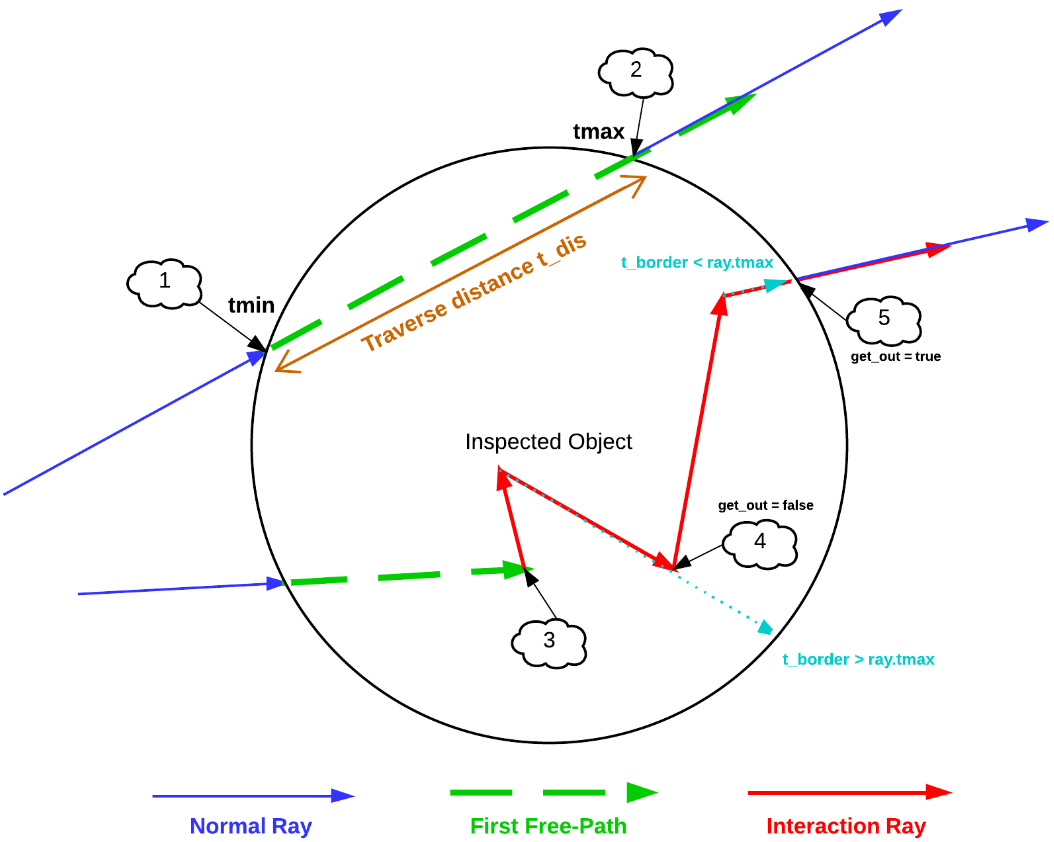
\includegraphics[width=\textwidth,height=\textheight,keepaspectratio]{Figures/model.png}
	\caption{OptiX photon interaction model.}%
	\label{fig:model}
\end{figure}\\

After learning the intersection mechanism of OptiX, we managed to solve this modeling problem. \fref{fig:model} points out the five essential procedures of this process:
\begin{enumerate}
  \item{
In \textit{Intersection Program}, a normal ray obtains its two \textit{t} values for intersecting a sphere object: \textit{tmin} and \textit{tmax}. Then \textit{Intersection Program} reports \textit{tmin} as the nearest intersection point and transfers the traversal distance \textit{t\_dis} to \textit{Normal Ray Closest Hit Program} by \textit{Attribute} semantic.
  }
  \item{
In \textit{Normal Ray Closest Hit Program}, CURAND is employed to generate the photon's first free-path \textit{pd.L}. If this path distance is greater than \textit{t\_dis}, it symbolizes that the photon has no interaction in the object. In this situation, a new normal ray will be emitted at the initial exit point.
\begin{lstlisting}[mathescape]
    // Cast a new normal ray at exit with the same direction
    Ray interaction_ray(exit, ray.direction,normal_type, scene_epsilon,RT_DEFAULT_MAX);
\end{lstlisting}
  }
  \item{
Otherwise (\textit{t\_dis} $<$ \textit{pd.L}), we update particle properties and produce a new free-path to replace the former one in \textit{Normal Ray Closest Hit Program}. Then, a new ray of type \textit{interaction\_type} will be launched with an up-to-date direction at the end of the first free-path. The trick in this process is to define the ray property \textit{tmax} with the new free-path.
\begin{lstlisting}[mathescape]
    // Cast new ray with interaction_type and tmax=pd.L
    Ray interaction_ray( hit_point, new_direction, interaction_type, scene_epsilon, pd.L );
\end{lstlisting}
  }
  \item{
An interaction ray calls \textit{Intersection Program} to determine potential crossing points as well. It will at first calculate a \textit{t\_border}, which represents a ray's minimum \textit{t} value to reach the sphere border. Afterwards, it will compare this \textit{t\_border} with the ray property \textit{tmax}. If \textit{tmax} is no bigger than \textit{t\_border}, which means the photon will stay in the sphere and continue to have other interactions, \textit{Intersection Program} will call \textit{Interaction Ray Closest Hit Program} at the end of \textit{tmax} and will signalize a flag \textit{get\_out=false} with \textit{Attribute}. The flag informs \textit{Interaction Ray Cloeset Hit Program} to launch a new ray that won't exit the object and the ray type is always \textit{interaction\_type}.
  }
  \item{
If \textit{tmax} exceeds \textit{t\_border}, the photon will arrive at the sphere border before it runs through the current free-path. At this time, \textit{Intersection Program} will invoke \textit{Interaction Ray Closest Hit Program} with the crossing point corresponding to \textit{t\_border}. The flag \textit{get\_out=true} informs \textit{Interaction Ray Closest Hit Program} that the next ray will escape from the sphere and there won't be interactions any more. So it needs to launch the following ray in \textit{normal\_type} and right on the border.
  }
\end{enumerate}
%----------------------------------------------------------------------------------------

\subsection{Object-Oriented Programming on GPUs}
As it has been indicated by \textit{CUDA Programming Guide} \citep{cudaguide}, CUDA supports full C++ for the host code but not for the device code, the same for OptiX. Consult \href{http://docs.nvidia.com/cuda/cuda-c-programming-guide/index.html#restrictions}{http://docs.nvidia.com/cuda/cuda-c-programming-guide/index.html\#restrictions} for more restriction details. Generally speaking, most of these restrictions are related to the CUDA streaming-processing architecture.

Actually, the main difficulty of object-oriented programming is that we should remove all dynamic allocations since it's not available on GPUs. Furthermore, this part of the code is relatively more hierarchical than other objects in MODERATO. All geometry objects locating in a file with 20000 lines of programs pressure the work as well.

In a word, creating user-defined objects in OptiX is feasible. Object-oriented programming allows us to adapt more easily complex geometry objects to OptiX.
%----------------------------------------------------------------------------------------
